
\subsection{Cosine Theta distribution}
\label{sec:cosine3D}
As mentioned in Sec.~\ref{sec:input}, the emission angle of photoelectrons in PyECLOUD is meant to follow a cosine distribution:
\begin{align}
    \derivative{n}{\Omega} &\propto \cos\theta
    \\
    \text{d}\Omega_{2D} &= \text{d}\theta
    \\
    \text{d}\Omega_{3D} &= \sin\theta~\text{d}\theta~\text{d}\varphi
    \label{eq:angles}
\end{align}
In PyECLOUD, the two-dimensional case is implemented even though the buildup process really happens in 3D space.
On average, this leads to too small angles (see Fig.~\ref{fig:distribution}), and is a common error in 2D simulation codes~\cite{angle}.
It impacts the buildup simulations because it influences the time necessary for a photoelectron to reach the opposing wall of the chamber, and potentially be absorbed there.
A branch on GitHub named "angle\_cosine3" changes this behavior.
%TODO
%
%

\begin{figure}[tbh]
    \centering
    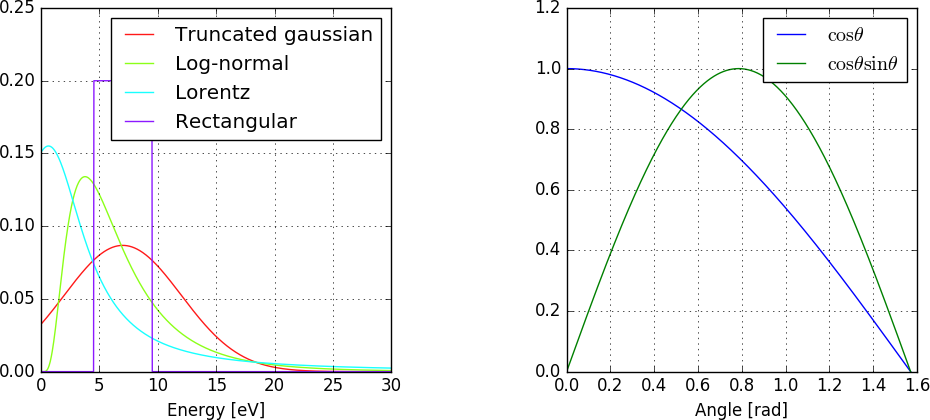
\includegraphics[width=0.8\textwidth]{../plots/distributions.png}
    \caption{
        The left plot shows a cut-off normal distribution characterized by a width and a standard deviation.
        A log-normal distribution with the same mean and variance as the undistorted Gaussian distribution is shown in green.
    The log-normal distribution does not extend to negative values.
    }
    \label{fig:distribution}
\end{figure}


\subsection{Delayed photoelectron production}
\label{sec:delay}

In PyECLOUD, photoelectrons are generated in parallel to the beam charge.
This means that the difference in path length is not considered.
Until a photon hits the chamber wall, the bunch has moved further due to the bending, see Fig.~\ref{fig:drawing}.
\begin{figure}[tbh]
    \centering
    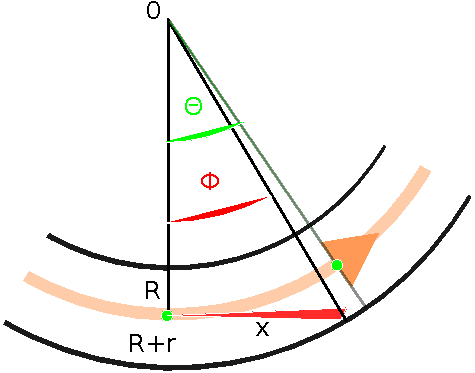
\includegraphics[width=0.5\textwidth]{../scripts/drawing.pdf}
    \caption{The path difference between protons (green) and photons(red).}
    \label{fig:drawing}
\end{figure}
The path difference is calculated in the following way, where $R=2803.95$~m for the LHC, and $r=22$~mm.
$x$ is the distance travelled by the photons before the wall is reached.
\begin{align}
    (R+r)^2 &= R^2 + x^2
    \\
    x &= \sqrt{2Rr + r^2} = 11.1~\text{m}
    \\
    \Phi &= \tan\frac{x}{R} = 0.00396136
    \\
    \Theta &= \frac{x}{R} = 0.00396134
    \\
    \Delta t &= \frac{R(\Theta - \Psi)}{c} = 1.938\cdot10^{-13}~s
\end{align}
This path difference is negligible as it is much smaller than a time step in the simulation, normally around $10^{-11}$~s.

Furthermore, photons that are absorbed only after (multiple) reflections (note that the reflection coefficient for grazing incident photons on Copper without sawtooth is larger than 80\%) are delayed with respect to the originating beam charge.
One reflection in normal direction causes to a delay of $\Delta t = \frac{2r}{c} = 1.48\cdot10^{-10}$~s, insignificant with respect to the bunch spacing of $2.5\cdot10^{-8}$, but longer than a time step in the simulations.
Backward or forward reflections, as indicated in Fig.~\ref{fig:synrad} could however lead to 
% TODO
% continuous photoemission


\subsection{Energy of new photoelectrons}

The energy of newly created photoelectrons is not very relevant in the current implementation of PyECLOUD, as they are immediately accelerated to much higher energies by the electric field of the beam charge.
If however a delayed photoemission was implemented, it could become more important.

The currently used truncated Gaussian for the energy distribution is not supported by laboratory measurements.
Other distributions have been introduced to the branch "photoemission", available on GitHub.
These are specified by the new input parameter \textbf{energy\_distribution}, which allows to choose from the following options in addition to the truncated Gaussian:
\begin{itemize}
    \item a log-normal distribution, which is also used for new secondary electrons.
        One advantage is that it does not have to be truncated, as negative energies cannot occur.
    \item a truncated Lorentzian, as indicated by Fig.~\ref{fig:cimino_cu_spectrum}.
        However it only fits well for the low-dose sample, otherwise the low-energy part is greatly reduced.
    \item a rectangular or a mono-energetic distribution in order to study the impact.
\end{itemize}
Figure~\ref{fig:distribution} visualizes the first three approaches, while Fig.~\ref{fig:test_energy_dist} shows a comparison of the resulting heat loads for different energy distributions, as well as the electron density
It shows that the initial energy of the photoelectrons hardly has an impact, at least with the current version of the code where photoelectrons are not created in between bunches.
Notable is the spike caused by the fat tail of the Lorentzian distribution, which is expected to generate photoelectrons with a very high energy from time to time, and should therefore be avoided.

\begin{figure}[tbh]
    \centering
    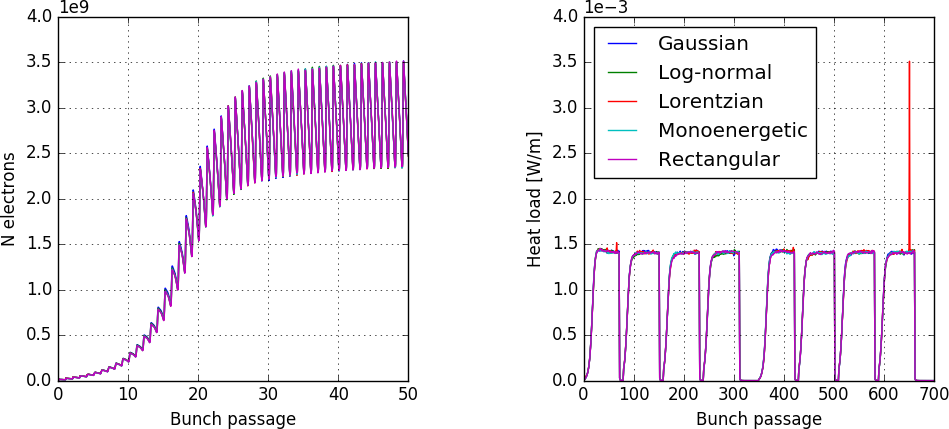
\includegraphics[width=0.8\textwidth]{../plots/energy_distribution_impact.png}
    \caption{
        The impact of several different energy distributions is compared for an e-cloud buildup simulation of the LHC chamber in a dipolar field at 6.5~TeV beam energy and nominal beam parameters.
        Left: The number of electrons in an electron-cloud buildup simulation.
        Right: The heat load per bunch passage.
    }
    \label{fig:test_energy_dist}
\end{figure}

Figure~\ref{fig:time} visualizes the time a photoelectron with a given energy and emission angle within the e-cloud stripes in a dipole needs to reach the opposing wall in absence of electric fields.
In the currently used photoemission module of PyECLOUD this hardly makes a difference as photoelectrons are created simultaneously with the bunch charge and are therefore immediately accelerated.
In case additional photoelectrons were created independent of time, or delayed with respect to the bunch, it may become relevant as low energy photoelectrons are more relevant because they do not reach the wall before the next proton bunch arrives and cannot get lost.

\begin{figure}[tbh]
    \centering
    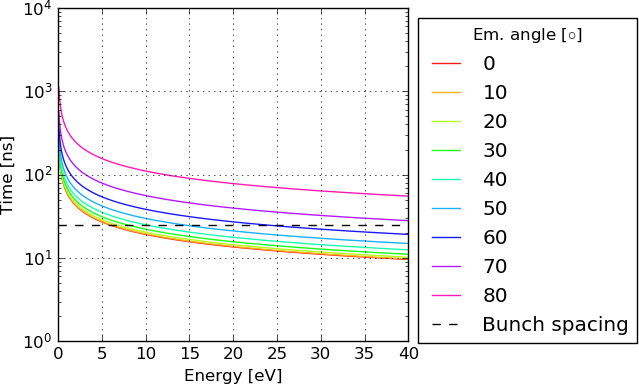
\includegraphics[width=0.55\textwidth]{../plots/time.png}
    \caption{The time needed for a photoelectron in a dipole e-cloud stripe to reach the opposing wall in dependence of the emission angle relative to the surface normal, in absence of electric fields.}
    \label{fig:time}
\end{figure}



\subsection{Distribution of photoelectrons in the chamber.}
\label{sec:photon_cdf}

Another idea would be to simulate the distribution of absorbed photons, and therefore the positions of new electron macroparticles.
So far, either a cosine squared or a uniform distribution of $\Psi$ in Fig.~\ref{fig:gt} has been used in most simulations.
Based on the high reflectivity of the non-sawtooth parts of the LHC chamber (at least for grazing incident angles), a uniform distribution might be the best approximation for the time being.

%For the log-normal distribution, the parameters $\sigma_l$ and $\mu_l$ have to be used in order to achieve the same sample variance and mean as for a normal distribution characterized by $\sigma_n$ and $\mu_n$.
%\begin{align}
%    \sigma_l &= \sqrt{\log\left(\frac{\sigma_n^2}{\mu_n^2}+1\right)}
%    \\
%    \mu_l &= \log\mu_n - \frac{\sigma_l^2}{2}
%\end{align}
%A branch called "photoemission" on GitHub adds a new input parameter \textbf{energy\_distribution}, the choices are in addition also a monoenergetic and a rectangular distribution.

